\section{Exact objectives and implementation}
\label{supp:losses}
\subsection{Autoencoder and full training objectives}
Let $X$ be a CT crop of $H\times W\times N_z$ voxels, $S_i$ its binary mask for
sheet $i$, and $P_i=\{p_k\}_{k=1}^{K}$ its $K$ positive prompt coordinates.
Here $H,W,N_z$ are the three spatial dimensions.
The AE encoder $E$ maps a corrupted mask $\widetilde S_i$ to a code $z_i$;
its occupancy decoder $D$ predicts probability $Q_i$:
\begin{equation}
 z_i=E(\widetilde S_i),\qquad Q_i=\sigmoid(D(z_i\odot(1+\xi))).
 \label{eq:ae}
\end{equation}
Here $\sigmoid$ is the logistic function, $\odot$ is elementwise multiplication,
and $\xi$ is independent uniform noise in $[-0.02,0.02]$ during AE training.
At $320^3$ input, the code is $64\times10^3$. No encoder--decoder skip
connections bypass it (Fig.~\ref{fig:ae}). The other heads predict a dense
unsigned distance field $U_i$, a distance $h(z_i,q)$ at query coordinate $q$,
and four intermediate occupancy maps $Q_i^{(a)}$.

Define $\mathcal L_{\rm seg}$ as weighted BCE plus soft Dice loss. The AE uses
\begin{align}
 \mathcal L_{\rm AE}={}&\mathcal L_{\rm seg}(Q_i,S_i)
   +\sum_a\alpha_a\mathcal L_{\rm seg}(Q_i^{(a)},S_i^{(a)})\nonumber\\
 &+\lambda_U\mathcal H(U_i,d_i)
  +\lambda_q\mathbb E_q\mathcal H(h(z_i,q),d_i(q))\nonumber\\
 &+\lambda_r\mathbb E_{i\ne j}[\relu(\cos(z_i,z_j)-m)]\nonumber\\
 &+\lambda_o R_o(Q_i,S_i)+\lambda_b R_b(Q_i,S_i).
 \label{eq:aeloss}
\end{align}
The index $a$ denotes decoder stages; $S_i^{(a)}$ is the resized target.
$\mathcal H$ is Smooth L1 loss, $d_i$ is unsigned distance to the sheet,
clipped at 16 voxels and divided by 16, and $d_i(q)$ is its sampled value.
The cosine term repels codes of distinct sheets in the same crop; $m=0.5$
is its margin and $\relu(t)=\max(t,0)$. $R_o$ and $R_b$ penalize foreground
outside a two-voxel GT tolerance and at the volume border. The $\alpha_a$ and
$\lambda$ symbols are loss weights, specified below. The sheet prior uses no explicit topology loss.

\subsection{Point-conditioned model and joint binary head}
The CT encoder $C$ produces a $512\times10^3$ grid and four context attention
blocks. Each prompt token combines Fourier coordinates, trilinearly sampled
CT features and its positive label. Prefix attention and four transformer
blocks $T$ predict the normalized sheet code (Fig.~\ref{fig:training}):
\begin{align}
 \bar z_i&=(E(S_i)-\mu)/\sigma,\qquad
 \widehat{\bar z}_i=T(C(X),P_i),\nonumber\\
 \widehat S_i&=\mathbf1[\sigmoid(D(\mu+\sigma\odot\widehat{\bar z}_i))\ge0.5].
 \label{eq:p2sd}
\end{align}
$\mu$ and $\sigma$ are fixed channel means and safe standard deviations of AE
codes; $\mathbf1$ is an indicator. The AE remains frozen. A separate binary
head $B$, with convolutional skip connections, predicts sheet union probability
$V=\sigmoid(B(C(X)))$ and supervises the shared CT features.

For transformer round $r$, let $\widehat{\bar z}_i^{(r)}$ denote its code, and
let $d(u,v)=\|u-v\|_2^2/L$ be MSE over $L$ code elements. Training minimizes
\begin{align}
 \mathcal L_{\rm train}={}&\sum_r\beta_r d(\widehat{\bar z}_i^{(r)},\bar z_i)
 +0.5\mathcal L_{\rm same}+0.25\mathcal L_{\rm diff}\nonumber\\
 &+\mathcal L_{\rm seg}^{\Omega}(V,Y),\label{eq:p2sdloss}\\
 \mathcal L_{\rm same}&=\mathbb E_{i,P}d(\widehat{\bar z}_{i,P},c_i),\nonumber\\
 \mathcal L_{\rm diff}&=\mathbb E_{i\ne j}[\relu(1-d(
 \widehat{\bar z}_i,\widehat{\bar z}_j))].\nonumber
\end{align}
$c_i$ is the mean code of same-sheet prompt sets $P$ in a batch. Different-sheet
pairs share a CT crop. $\beta=(0,0.5,1,1)$ weights the four rounds; $Y$ is the
GT binary union and $\Omega$ its non-ignored voxels. The binary loss uses
positive BCE weight 2 and soft Dice on $160^3$ crops. Point-to-sheet training
uses no decoded occupancy loss in the main model.


\subsection{Connections between the AE modules}
Figure~\ref{fig:ae_modules} expands the AE heads and their supervision.
The reference dense encoder begins with a factor-four patch stem, followed
by stage-matched residual convolutions and downsampling to a $10^3$ grid.
The code has 64 channels. The implementation also retains an occupied-voxel
sparse encoder for future efficiency experiments; it densifies its bottleneck
for the same decoder and heads. It is not used by the reported checkpoints.

The dense decoder applies five residual/convolutional upsampling stages,
with spatial sizes $10,20,40,80,160,320$ and channels
$64,48,32,24,16,8$. Final $1\times1\times1$ heads predict occupancy logits
and unsigned distance. Four intermediate occupancy heads attach at spatial
sizes $20,40,80,160$. The query head instead samples the noisy code at a
query coordinate, concatenates normalized coordinates, and applies a
width-128 MLP. There are no encoder--decoder skip connections.

\begin{figure*}[t]
 \centering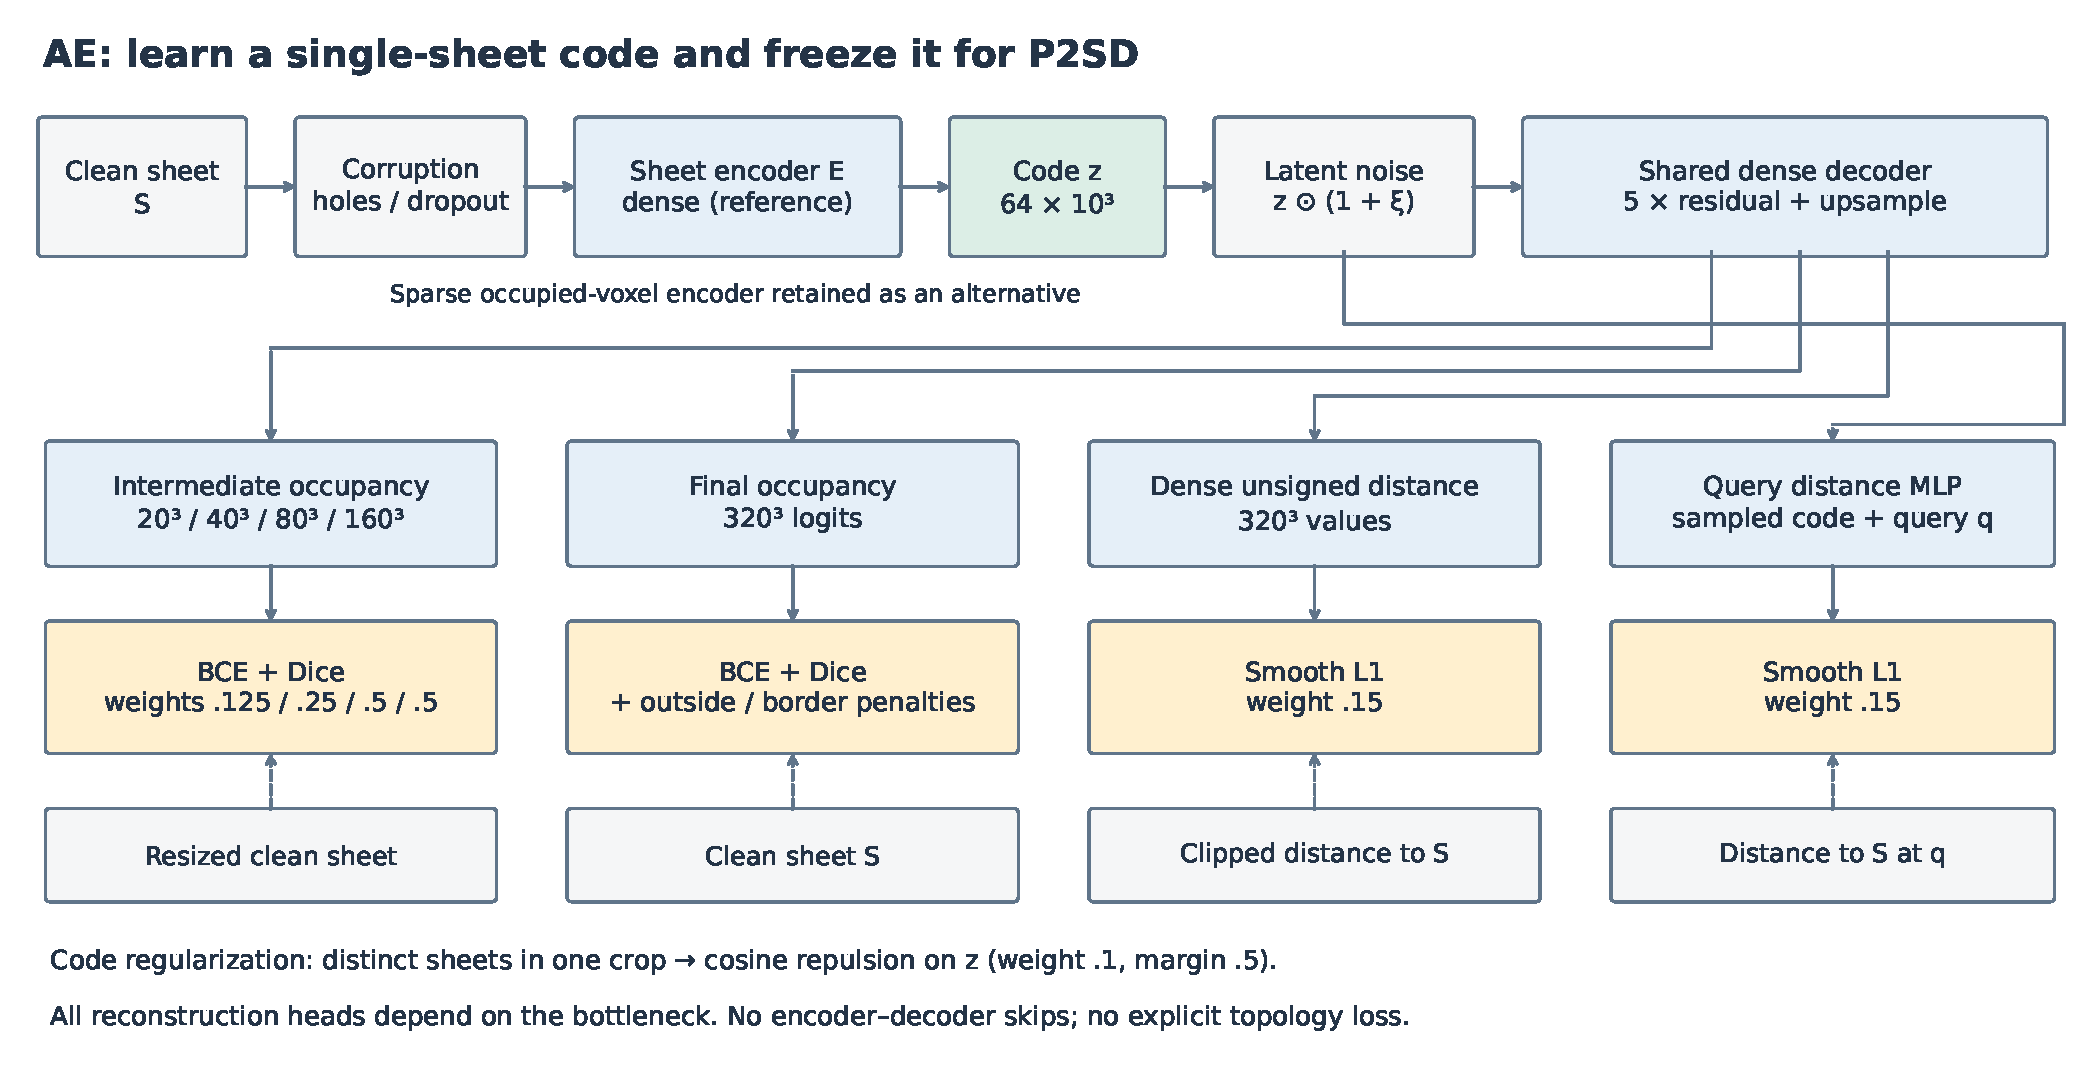
\includegraphics[width=\textwidth]{figures/ae_modules.pdf}
 \caption{\textbf{AE modules and supervision.} Decoder occupancy and distance
 heads share dense features; query distance is predicted directly from the
 noisy latent code. Each loss is paired with its target. Intermediate heads
 attach at successive decoder stages. Code repulsion acts on distinct-sheet
 codes before latent noise. The sparse encoder remains an optional alternative.}
 \label{fig:ae_modules}
\end{figure*}

\subsection{Connections between the P2SD modules}
Figure~\ref{fig:p2sd_modules} separates shared image computation from
prompt-dependent computation. The image encoder reduces CT to a
$512\times10^3$ feature grid. A $1\times1\times1$ projection and four
self-attention blocks form the image context $F$: 1,000 tokens of width 512.
Three-dimensional per-axis rotary coordinates supply position information.

For each prompt coordinate $p_k$, prompt composition concatenates its
eight-band Fourier encoding, the trilinearly sampled context $F(p_k)$,
and the positive-label scalar. A two-layer MLP produces one width-512 token
per point. The reference retains all $K$ prompt tokens. The prompt modulator
prefixes them to the context tokens, aligns their coordinate frames for
rotary attention, and applies one attention block. Prompt-prefix outputs
are discarded; the remaining 1,000 conditioned grid tokens enter the refiner.

The refiner contains four self-attention blocks with eight heads and SwiGLU
MLPs. Linear projections supply intermediate code estimates; a separate
LayerNorm and linear projection supply the final normalized 64-channel code.
The loss distinguishes these auxiliary projections from the final head, as
specified in Eq.~\ref{eq:p2sdloss}. Channel statistics come from training-sheet
AE codes. Inference reverses this normalization before the frozen AE decoder.

The binary branch receives the \emph{unprompted} image context, applies its
own four attention blocks, and upsamples with residual/convolutional stages
of channels $512,256,128,64,32,16$. A final $1\times1\times1$ head produces
union logits. It has no encoder--decoder skip connections; residual
connections inside individual blocks are distinct. Its loss updates the
shared image encoder and image-context blocks. In the new training recipe,
refinement sees the complete $10^3$ context and decoding builds the full
$160^3$ intermediate feature grid. We crop $80^3$ features there and apply
the final $\times2$ upsampling, residual block and occupancy head to obtain
$160^3$ output supervision. Earlier stages retain full-volume context at
increased activation-memory cost. This is the retained \texttt{second\_last}
crop mode, also used by 0076. The scored 0058 checkpoint instead used an
earlier $5^3$ context crop; its measurements are unchanged.

\begin{figure*}[t]
 \centering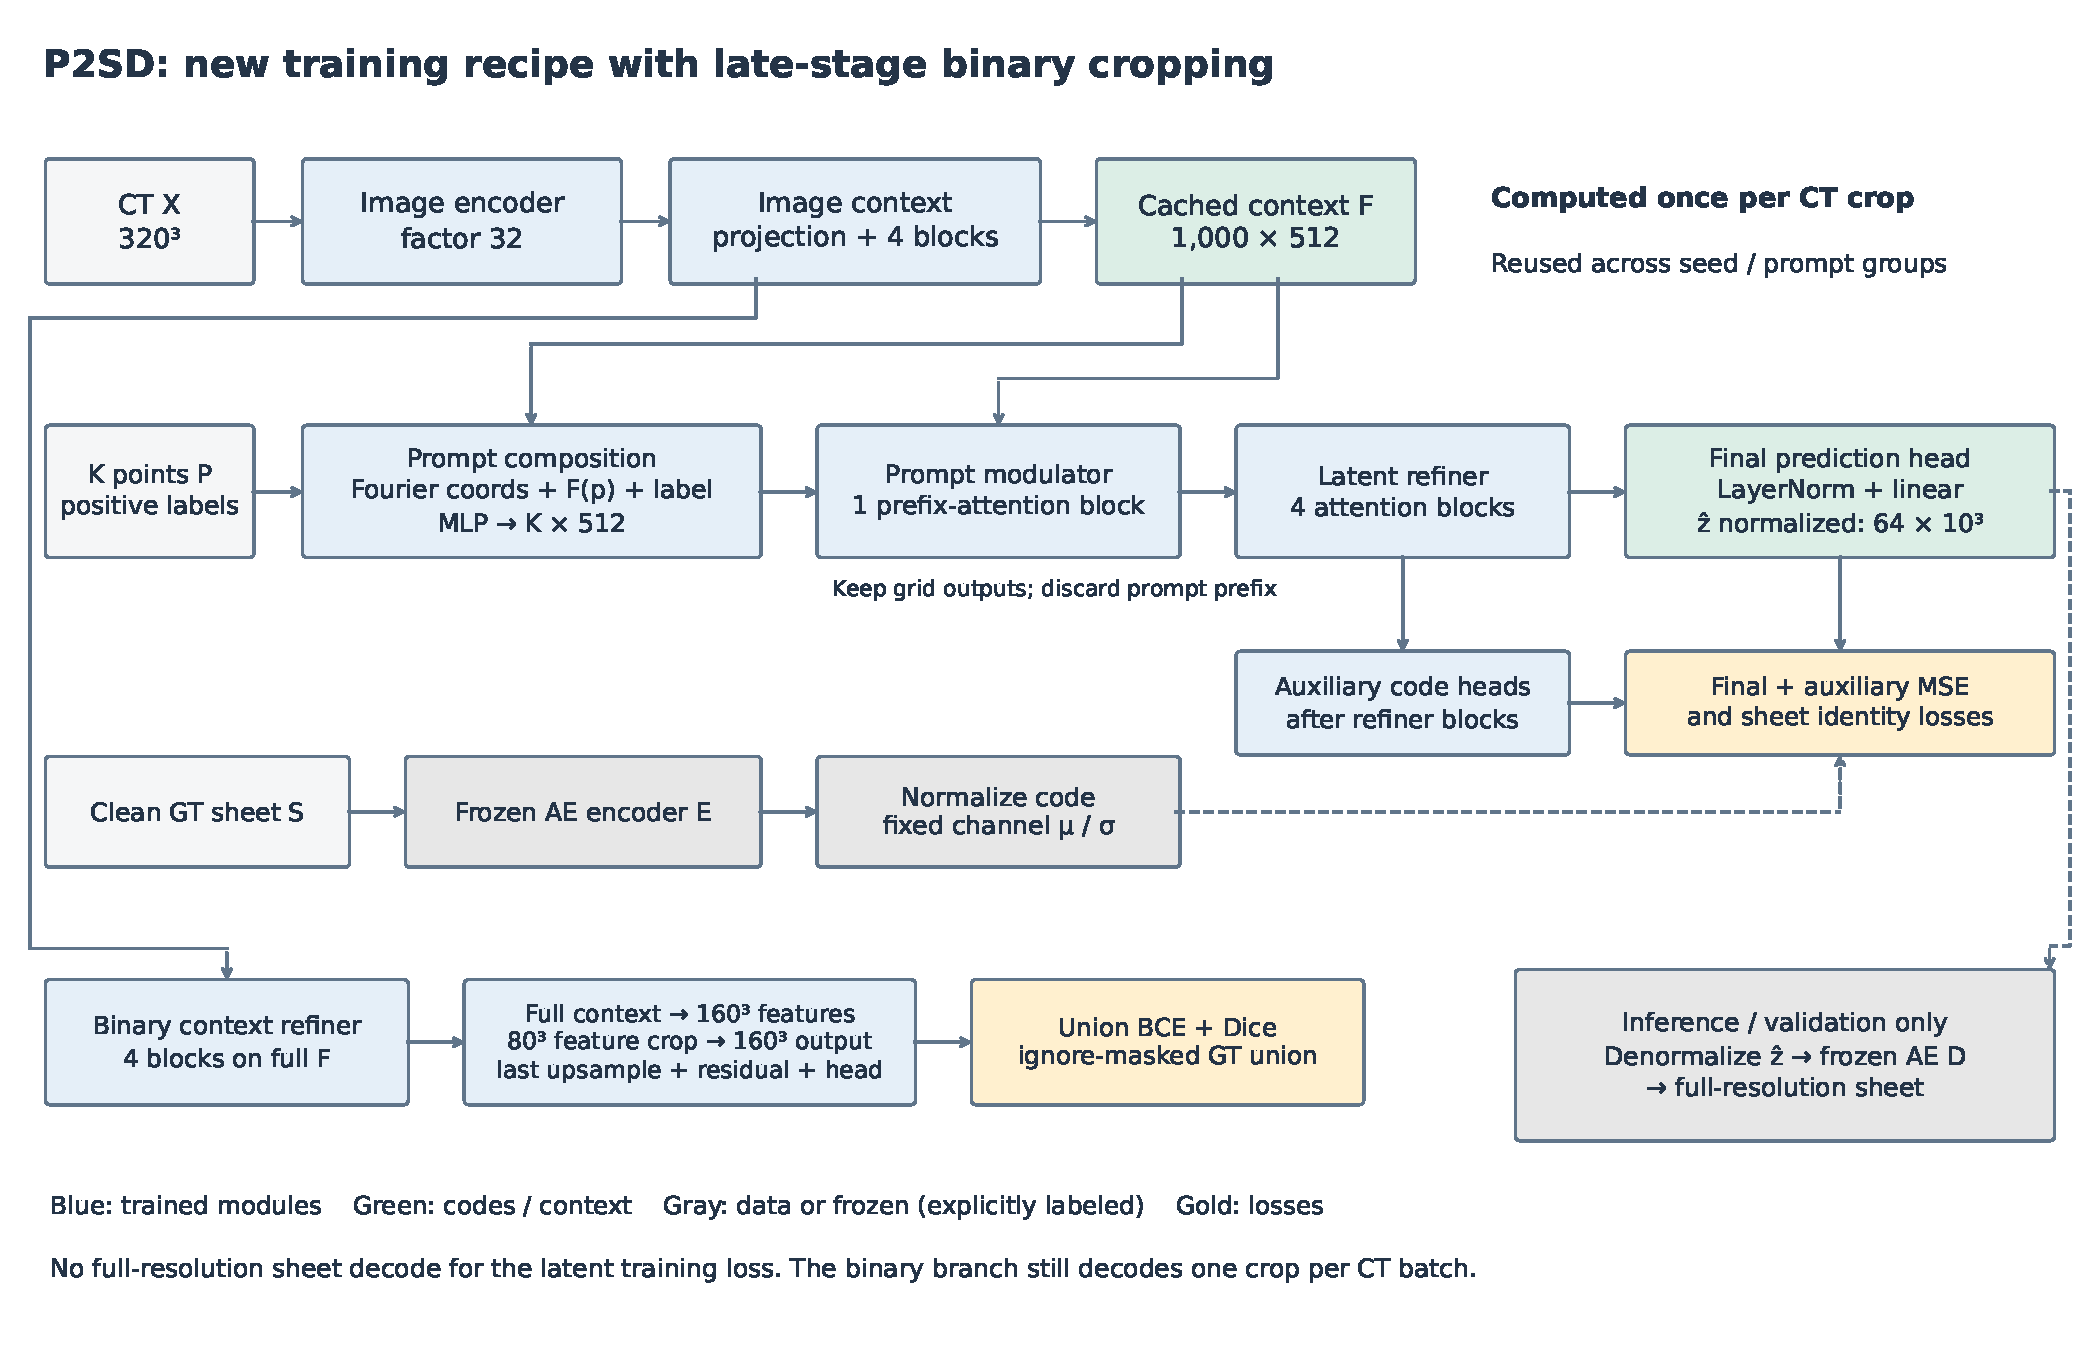
\includegraphics[width=\textwidth]{figures/p2sd_training_recipe.pdf}
 \caption{\textbf{P2SD modules in the new training recipe.} Shared CT encoding
 and context feed prompt composition, modulation and refinement. Code heads
 learn from the frozen AE. The binary branch decodes full context to $160^3$
 features before cropping for its final upsampling; at inference it decodes
 the full union for seed proposal. The sheet decoder is used only when masks
 are needed under the main latent objective. Optional query losses are
 described separately; the scored 0058 checkpoint used earlier cropping.}
 \label{fig:p2sd_modules}
\end{figure*}

\subsection{Efficiency of compact latent prediction}
For a $320^3$ crop, prompt conditioning and code prediction operate on only
$10^3=1{,}000$ spatial sites, compared with $32{,}768{,}000$ output voxels.
Including its 64 channels, a sheet code has 64,000 scalars, 512 times fewer
than one full-resolution scalar mask. At BF16, these tensors occupy
0.122 MiB and 62.5 MiB, respectively; the shared $512\times10^3$ context
occupies 0.977 MiB. These are tensor-size comparisons, not measured speedups
or total training-memory estimates. Attention still incurs token-pair work.

Let $N$ be the number of foreground seeds, $G$ the number of additional
multi-point prompt groups used for cluster consistency, and $K$ the number
of sheet hypotheses that are densely decoded. Let $C_{\rm img}$ denote
shared CT encoding/context cost, $C_{\rm code}$ the cost per prompt group,
$C_{\rm cluster}$ clustering cost, $C_B$ the binary branch's refinement and
union decoding cost, and $C_D$ one AE decoding cost. With the co-trained
proposal head, automatic inference has approximate cost
\begin{equation}
 C_{\rm img}+C_B+(N+G)C_{\rm code}+C_{\rm cluster}+K C_D.
\end{equation}
This avoids paying a full upsampling cost for each of the $N$ seed codes
before clustering. Retained sheets still require dense decoding, output
storage and cleanup. The co-trained proposal head reuses the cached image
context and incurs one full-resolution union decode. The historical benchmark
instead uses a separate proposer with its own CT encoder, so its cost includes
an additional encoding. No binary training crop is applied at inference.

During P2SD training, the frozen teacher encoder produces sheet targets, but
the active latent objective does not require AE decoding. The auxiliary
binary branch still decodes a crop once per CT batch, and validation decodes
full sheet masks. We therefore claim an architectural advantage in repeated
prompt processing, rather than an unmeasured end-to-end runtime advantage.

\subsection{Loss definitions and architecture settings}
For a probability map $Q$, binary target $S$, valid voxel set $\Omega$ and
positive BCE weight $\omega$, the segmentation loss in the main text is
\begin{align}
 \mathcal L_{\rm seg}^{\Omega}&=\mathcal L_{\rm BCE}^{\Omega}
                                  +\mathcal L_{\rm Dice}^{\Omega},\nonumber\\
 \mathcal L_{\rm BCE}^{\Omega}&=-\frac{1}{|\Omega|}\sum_{v\in\Omega}
 \left[\omega S_v\log Q_v+(1-S_v)\log(1-Q_v)\right],\nonumber\\
 \mathcal L_{\rm Dice}^{\Omega}&=1-
 \frac{2\sum_{v\in\Omega}Q_vS_v+\epsilon}
 {\sum_{v\in\Omega}Q_v+\sum_{v\in\Omega}S_v+\epsilon}.
 \label{eq:segexact}
\end{align}
$Q_v=Q(v)$ and $S_v=S(v)$; $v$ indexes voxels and $\epsilon=10^{-6}$ stabilizes the Dice ratio.
Without the superscript, all voxels are valid. AE BCE uses
$\omega=\min(20,\max(1,N_-/\max(N_+,1)))$, where $N_+$ and $N_-$ count
foreground/background voxels in the training batch. Intermediate targets use
max pooling to the head resolution. The joint binary head uses $\omega=2$;
ignore is removed from both Dice sums, and empty-target crops contribute BCE
but are excluded from the batch Dice average.

In Eq.~\ref{eq:aeloss}, the four intermediate weights are
$\alpha=(0.125,0.25,0.5,0.5)$ and
$(\lambda_U,\lambda_q,\lambda_r,\lambda_o,\lambda_b)
=(0.15,0.15,0.1,0.05,0.05)$.
Smooth L1 uses transition width 0.1 and averages over dense voxels or query
samples. The penalties are
\begin{equation}
 R_o=\frac{\sum_{v\notin\operatorname{dilate}_2(S)}Q(v)}{\max(|S|,1)},\qquad
 R_b=\frac{\sum_{v\in\partial_5}Q(v)}{\max(|S|,1)}.
\end{equation}
$\operatorname{dilate}_2$ is a cubic two-voxel dilation and $\partial_5$ is the
five-voxel crop border. Cosine similarity flattens the latent tensor.
AE input corruption is applied with probability 0.7: one to six spherical
holes of radius 2--10 voxels and dropout up to 0.3, retaining at least 25\%
of the sheet. The unsigned-distance query head uses 8,192 queries.

The AE uses convolutional channels $(8,16,24,32,48,64)$, RMS normalization,
and factor-32 reduction; its distance-query MLP has width 128.
The CT encoder channels are $(16,32,96,192,384,512)$, with an early
factor-four stem. Point Fourier encoding has eight bands. Context and
point-refinement attention each have four blocks, 512-dimensional features
and per-axis rotary coordinates; refinement uses eight heads.
The joint binary branch has its own four-block refiner and convolutional
decoder channels $(512,256,128,64,32,16)$. Dense auxiliary training decodes
$5^3$ context crops into $160^3$ masks, while sheet codes retain the $320^3$
crop extent. All main-model checkpoint, configuration and latent-statistics
hashes accompany the result snapshot.
The AE and main CT model use Kaggle-derived t6 training labels with topology
repair/cleanup; external scroll labels are excluded from the main model.
Evaluation uses the released test annotations, not those repaired training
labels. Training-ID exclusion alone does not certify spatial disjointness.
Cached CT inputs share five-voxel image-border zeroing; GT borders are retained.

\section{Automatic clustering and instance diagnostics}
\paragraph{Figure 3: measured inference intermediates.}
We reuse case 00860 and its central native $z=160$ section, as in the binary
failure example. The frozen automatic run provides all 512 seed coordinates,
foreground and final instances. A forward replay with the same 0058 checkpoint,
BF16 precision and seed batch size 32 captures the CT context and all
64,000-dimensional point codes. Replayed retained-cluster sizes match the
saved inference log. Colors identify final instances after duplicate handling,
so multiple retained clusters may share a color. Gray codes belong to discarded
clusters; their exclusion is not hidden from the plot.
CT seed markers use the $z\pm12$ slab for visibility, whereas the CT and mask
images use the exact central plane. The feature panel shows channel RMS of
the cached $10^3$ CT context at the corresponding depth, without interpolation.
The code panel uses deterministic PCA over all 512 codes; its two components
explain 27.8\% of variance. This projection is for display only: the algorithm
clusters in full code space. It need not visibly separate all sheet identities.
Native arrays, point codes, assignments and source hashes accompany the figure.

\paragraph{Measured latent identity separation.}
Each of the eight fixed GT coordinates per band is queried separately, yielding
6,112 single-point codes across all 106 cubes. Distance uses the complete
normalized code, without decoding or threshold calibration. GT connected bands
provide analysis identities, rather than physical-sheet guarantees.
On 106 cases and 6,112 fixed GT points, the median same-band MSE is 0.0201, versus 2.1280 between bands. Pair AUROC is 0.9121; mean per-case nearest-band accuracy is 80.80\%. At the inherited 0.02 threshold, 50.03\% of same-band pairs exceed the threshold and 1.31\% of different-band pairs fall below it.

The same-band p90 is 1.682, so the tails overlap substantially despite separated
medians. These spatially spread GT points include difficult crop-edge locations
and differ from the automatic foreground-seed distribution. Pairwise rejection
is not the fraction of points excluded by leader clustering; nearest-neighbor
links and cluster means affect assignment. Results support useful separation
while identifying remaining point-conditioning errors.

The controlled foreground proposer is frozen model 0022, shared across all
checkpoints; it is separate from their jointly trained binary heads.
Foreground probability threshold is 0.6, with 512 uniformly sampled voxels.
One cached CT context serves all single-point latent predictions. Sequential
leader clustering joins the nearest cluster mean at latent MSE $\le0.02$;
otherwise it creates a new cluster. Clusters with eight or fewer points are
discarded. For seven eight-point subset predictions $u_t$, define
\begin{equation}
 r_t=\min_{s\ne t}d(u_t,u_s),\qquad r_{\min}=\min_t r_t.
\end{equation}
Here $s,t\in\{1,\ldots,7\}$ index subsets, and $d$ is normalized latent MSE
as in the main text. Candidates with $r_{\min}>0.008$ are discarded;
otherwise all seven codes are averaged and decoded once at threshold 0.5.
The rule checks subset agreement, not certified physical identity.

Each automatic decode retains its largest six-connected component.
Three-voxel dilation with overlap-cover threshold 0.2 suppresses duplicate
masks; predicted probability assigns contested voxels, and final IDs below
500 voxels are removed. Thus the automatic benchmark includes cleanup,
whereas raw prompted topology does not. Both small and unstable point clusters
are excluded from reconstruction. Leader order and fixed latent thresholds
remain limitations.

Tables~\ref{tab:auto} and~\ref{tab:autoinst} retain all automatic checkpoint
results on the 106 cases. The unfiltered common-foreground CC6 baseline is
not a matched-cleanup architecture ablation. Instance accuracy at IoU threshold
$\tau$ is TP/(TP+FP+FN), using greedy one-to-one annotated-band matching;
TP, FP and FN are matched predictions, unmatched predictions and missed bands.
It is not integrated AP. GT-normalized IoU sums matches at 0.5 and assigns zero
to unmatched GT bands. Merges count predicted majority-overlap claimants for
multiple GT bands; splits count GT bands receiving multiple majority claimants.
Annotation components are proxies, not certified physical-sheet identities.

\begin{table*}[t]
\centering
\small
\setlength{\tabcolsep}{4pt}
\begin{tabular}{lrrrrr}
\toprule
Arm & Dice & Surface Dice & TopoScore & VOI & Formula \\
\midrule
Foreground CC6 & 0.4191 & 0.7377 & 0.0883 & 0.5358 & 0.4722 \\
0058 & 0.4262 & 0.7494 & 0.2644 & 0.5396 & 0.5305 \\
0076 & 0.3847 & 0.6863 & 0.2269 & 0.5426 & 0.4982 \\
0076+100k & 0.3981 & 0.7098 & 0.2386 & 0.5403 & 0.5091 \\
\bottomrule
\end{tabular}
\caption{Completed automatic segmentation on 106 cubes under original source ignore. One common foreground and the same 512 sampled points are used for every P2SD checkpoint. The CC6 baseline labels the foreground directly.}
\label{tab:auto}
\end{table*}

\begin{table*}[t]
\centering
\small
\setlength{\tabcolsep}{4pt}
\begin{tabular}{lrrrrrrr}
\toprule
Arm & Acc$_{.25}$ & Acc$_{.50}$ & GT IoU$_{.50}$ & Pred & GT & Merges & Splits \\
\midrule
Foreground CC6 & 0.031 & 0.007 & 0.038 & 299.953 & 7.642 & 1.189 & 0.000 \\
0058 & 0.420 & 0.071 & 0.057 & 6.821 & 7.642 & 0.330 & 0.000 \\
0076 & 0.386 & 0.064 & 0.048 & 6.217 & 7.642 & 0.302 & 0.000 \\
0076+100k & 0.385 & 0.059 & 0.046 & 6.396 & 7.642 & 0.321 & 0.000 \\
\bottomrule
\end{tabular}
\caption{Per-case means of annotated-band instance diagnostics. Acc$_\tau$ is TP/(TP+FP+FN) at IoU $\tau$, not integrated AP. GT IoU sums IoUs of matches at threshold 0.50 and divides by the GT count, assigning zero to unmatched bands. Pred/GT are counts; merge and split definitions are those of the inherited matching implementation.}
\label{tab:autoinst}
\end{table*}


\section{External data and continued training}
\label{supp:checkpoints}
The two additional checkpoints investigate whether large-scale external data
and prolonged training help generalization to new scrolls.
\textbf{0076} initializes from Kaggle-only 0058 and adds mesh-derived
scroll patches, totaling 10,347 spatially overlapping training patches.
It adds latent coordinate-distance supervision, with query emphasis near mesh
vertices. \textbf{0076+100k} continues for 100,000 steps with geometric
consistency. All three retain the same frozen AE. Changed data, objectives and
training duration prevent a causal attribution to any one factor.

For the mixed-data query term, the frozen AE head $h$ supplies a teacher
prediction at query $q$ from clean code $E(S_i)$; Smooth L1 regresses the predicted
code's query output toward that teacher. The continuation additionally compares
aligned decoded probabilities under flips and right-angle rotations:
\begin{equation}
 \mathcal L_{\rm geo}=1-
 \frac{2\langle A_g,B_g\rangle+1}{\|A_g\|_2^2+\|B_g\|_2^2+1}.
\end{equation}
$A_g$ and $B_g$ are original/transformed $160^3$ probability blocks after inverse
alignment; inner products and norms sum voxels. A nonidentity transform is
sampled each step from the 16-element in-plane dihedral and axial-flip group.
Corresponding $5^3$ code crops are decoded, with gradients through both branches
and the frozen decoder. The consistency weight is 0.5.
AdamW uses stem, encoder, dense-head and other learning rates
$10^{-6},3\times10^{-6},10^{-5},5\times10^{-6}$, weight decay 0.02,
1,000 warmup steps and cosine decay to 10\% of their initial rates.
These settings allow intermediate checkpoint evaluation without relying on a
near-zero terminal learning rate.

\section{Full prompt-count and topology results}
Of the 106 released test cubes, 102 are $320^3$ and four are $256^3$.
Training-case IDs are disjoint; this does not establish spatial disjointness
within a scroll. The first-place baseline uses its released four-model
ensemble and postprocessing unchanged; only GPU routing is adapted.
Across 764 raw eight-point sheet predictions, mean $(b_0,b_1,b_2)$ is
$(1.183,0.165,0)$. After source-ignore erasure, mean $b_0$ rises to 22.857
and mean $b_1$ to 32.191. These whole-mask counts differ from matched TopoScore.
Here $b_0,b_1,b_2$ count components, tunnels and cavities under six-connected
foreground. In the selected binary failure crop, the raw winner union has
125 tunnels and the automatic PLatS union has three; this example is diagnostic,
not a representative estimate.

Eight spatially spread positive GT points are fixed per eligible annotated
band, with nested prefixes $K\in\{1,2,4,8\}$ identical across checkpoints.
The complete matrix has $3\times4\times764=9,168$ sheet tuples and 1,272
checkpoint/prompt/case unions. Smaller native cubes are centered with
32-voxel padding; masks, points and scores are cropped back. Every tuple has
aligned image, prompt, GT, prediction and ignore NIFTIs.

The prompted diagnostic ignores only the exterior of the rectangular
annotated-region box, retaining source-ignore regions \emph{inside} that box
as GT background. This avoids inward erasure cuts but is distinct from the
standard LB and restoration tables in the main text. Raw masks receive no
cleanup. Union GT includes annotated bands below the 10,000-voxel prompt
eligibility threshold. Tables~\ref{tab:promptmatrix} and~\ref{tab:unionmatrix}
retain Dice and all three formula terms for every prompt count.

\begin{table*}[t]
\centering
\small
\setlength{\tabcolsep}{4pt}
\begin{tabular}{lrrrrrr}
\toprule
Checkpoint & Points & Dice & SD$_2$ & Topo & VOI & Formula \\
\midrule
0058 & 1 & 0.4314 & 0.7689 & 0.6864 & 0.7502 & 0.7376 \\
0058 & 2 & 0.4329 & 0.7735 & 0.6994 & 0.7507 & 0.7433 \\
0058 & 4 & 0.4471 & 0.7936 & 0.6954 & 0.7463 & 0.7476 \\
0058 & 8 & 0.4517 & 0.8058 & 0.7045 & 0.7440 & 0.7538 \\
0076 & 1 & 0.4050 & 0.7445 & 0.6576 & 0.7557 & 0.7224 \\
0076 & 2 & 0.4115 & 0.7564 & 0.6546 & 0.7530 & 0.7247 \\
0076 & 4 & 0.4287 & 0.7820 & 0.6635 & 0.7477 & 0.7344 \\
0076 & 8 & 0.4334 & 0.7987 & 0.6772 & 0.7450 & 0.7435 \\
0076+100k & 1 & 0.4214 & 0.7621 & 0.6729 & 0.7505 & 0.7313 \\
0076+100k & 2 & 0.4269 & 0.7718 & 0.6658 & 0.7485 & 0.7319 \\
0076+100k & 4 & 0.4413 & 0.7939 & 0.6719 & 0.7446 & 0.7400 \\
0076+100k & 8 & 0.4422 & 0.8071 & 0.6821 & 0.7430 & 0.7472 \\
\bottomrule
\end{tabular}
\caption{Complete sheet results: all three checkpoints, all four nested prompt counts. Annotated-box ignore; no prediction cleanup. Formula scores are diagnostics under this policy.}
\label{tab:promptmatrix}
\end{table*}

\begin{table*}[t]
\centering
\small
\setlength{\tabcolsep}{4pt}
\begin{tabular}{lrrrrrr}
\toprule
Checkpoint & Points & Dice & SD$_2$ & Topo & VOI & Formula \\
\midrule
0058 & 1 & 0.4437 & 0.7922 & 0.5848 & 0.5336 & 0.6395 \\
0058 & 2 & 0.4465 & 0.7978 & 0.6054 & 0.5352 & 0.6482 \\
0058 & 4 & 0.4582 & 0.8132 & 0.6264 & 0.5343 & 0.6595 \\
0058 & 8 & 0.4619 & 0.8221 & 0.6171 & 0.5341 & 0.6598 \\
0076 & 1 & 0.4166 & 0.7692 & 0.5597 & 0.5296 & 0.6225 \\
0076 & 2 & 0.4220 & 0.7787 & 0.5373 & 0.5322 & 0.6200 \\
0076 & 4 & 0.4368 & 0.7994 & 0.5704 & 0.5335 & 0.6376 \\
0076 & 8 & 0.4426 & 0.8122 & 0.5990 & 0.5305 & 0.6497 \\
0076+100k & 1 & 0.4313 & 0.7836 & 0.5781 & 0.5308 & 0.6335 \\
0076+100k & 2 & 0.4370 & 0.7928 & 0.5543 & 0.5342 & 0.6308 \\
0076+100k & 4 & 0.4495 & 0.8114 & 0.5725 & 0.5349 & 0.6430 \\
0076+100k & 8 & 0.4512 & 0.8210 & 0.6065 & 0.5313 & 0.6553 \\
\bottomrule
\end{tabular}
\caption{Complete union results: all three checkpoints, all four nested prompt counts. Annotated-box ignore; no prediction cleanup. Formula scores are diagnostics under this policy.}
\label{tab:unionmatrix}
\end{table*}

\begin{table*}[t]
\centering
\small
\setlength{\tabcolsep}{4pt}
\begin{tabular}{lrrrrrrr}
\toprule
& \multicolumn{3}{c}{Per-sheet means} & & \multicolumn{3}{c}{Union means} \\
Checkpoint & $b_0$ & $b_1$ & $b_2$ & $P_{100}$ & $b_0$ & $b_1$ & $b_2$ \\
\midrule
0058 & 1.183 & 0.165 & 0.000 & 87.30\% & 8.179 & 63.292 & 9.528 \\
0076 & 1.385 & 0.658 & 0.263 & 81.94\% & 9.594 & 19.906 & 3.557 \\
0076+100k & 1.308 & 0.534 & 0.211 & 82.46\% & 8.953 & 40.302 & 5.896 \\
GT & 1.000 & 0.001 & 0.001 & 99.74\% & 7.642 & 0.009 & 0.009 \\
\bottomrule
\end{tabular}
\caption{Whole-mask raw Betti counts before scoring erasure or component cleanup. Sheet statistics cover 764 eligible bands; union statistics cover 106 cases. $P_{100}$ denotes the fraction of sheets with $(b_0,b_1,b_2)=(1,0,0)$. These counts do not replace spatial feature matching.}
\label{tab:topology}
\end{table*}


Table~\ref{tab:topology} counts raw topology before erasure. All three median
per-sheet vectors are $(1,0,0)$, while mean union tunnel counts expose outlier
contacts between decoded sheets. For 0058 the mean raw union $b_1$ is 63.292
but its median is one: mean counts must not be read as typical defects per
crop. The GT component construction also favors disk-like masks.
$P_{100}$ denotes fraction $(1,0,0)$ and is not proof of geometric correctness.
Exact TopoScore uses spatial Betti matching over eight crop octants, not a
comparison of whole-mask counts alone.
Our compact exact implementation reduces storage without approximating the
matching calculation. Formula arithmetic, 106-case coverage, native prompt
membership and unchanged checkpoint hashes are verified. Paired bootstrap
results average sheets within each case and resample 106 cases 2,000 times
(seed 42); source files preserve all intervals. Spatial dependence and prior
inspection limit their statistical interpretation.

\section{Restoration controls and failure provenance}
Preserve each predicted identity \emph{before} erasure. Let $A_i$ be its full
mask, $I$ the source-ignore mask, and $v_i=|A_i\setminus I|$ its visible size.
The restored, filtered binary union is
\begin{equation}
 A^{\rm rest}=\bigcup_{i:\ v_i>0,\ |A_i|\ge5000} A_i,\qquad
 J_{\rm rest}=J(A^{\rm rest},G\setminus I).
 \label{eq:restore}
\end{equation}
$|\cdot|$ denotes voxel count. Entirely ignored instances are excluded; the
5,000-voxel gate uses \emph{full size after restoration}. GT remains erased,
and restored predictions are not erased a second time. For the binary winner,
identities are its raw six-connected components; PLatS supplies predicted IDs.
The rule uses no GT foreground to select or complete a prediction.
Table~\ref{tab:modified} reports the same three formula terms after this change.
This is \emph{not official LB}: restored foreground can be penalized against
unknown GT background, and raw binary components are imperfect sheet proxies.
Filtering-only controls and a topology-isolation diagnostic are in Supplementary.


\begin{table*}[t]
\centering
\small
\setlength{\tabcolsep}{4pt}
\begin{tabular}{lrrrr}
\toprule
Method & Standard LB & Filter only & Restore + filter & Topology-only diagnostic \\
\midrule
Winner & 0.6176 & 0.6176 & 0.6537 & 0.6753 \\
PLatS auto & 0.5305 & 0.5304 & 0.6124 & 0.6257 \\
PLatS GT8 union & 0.5627 & 0.5627 & 0.6598 & 0.6611 \\
\bottomrule
\end{tabular}
\caption{Ignore-restoration controls. GT8 union uses deterministic sheet-ID ownership on overlaps and retains its original union exactly. It uses GT prompts and is not an automatic discovery result. The topology-only hybrid replaces only TopoScore.}
\label{tab:restorecontrols}
\end{table*}

The filtering-only control erases ignore after applying the same full-size
ID gate. The full restoration metric is Eq.~\ref{eq:restore}, including any
Surface Dice or VOI penalties for retained unknown foreground. To isolate the
changed topology term, we additionally report
\begin{align}
 J_{\rm topo\text{-}only}={}&0.35\,\mathrm{SD}_2(A^{\rm rest}\setminus I,G')\nonumber\\
 &+0.30\,\mathrm{Topo}(A^{\rm rest},G')\nonumber\\
 &+0.35\,\mathrm{VOI}(A^{\rm rest}\setminus I,G').
\end{align}
where $G'=G\setminus I$. This hybrid is a separate non-official diagnostic;
it is not the modified LB table in the main paper.

Failure examples use saved masks, never synthetic surfaces. The binary example
uses a visually clear lamellar CT cross-section among the top 20 cached
winner merger candidates. The central TIFF-stack slice is used, with a
four-connected winner region joining distinct GT bands. The ignore example maximizes induced tunnel count among raw $(1,0,0)$
0058 masks with visible support. Source hashes, selection metadata, native
voxels and slice coordinates are saved in the failure-analysis run. Selection
is diagnostic, not random or representative. Figures 4 and 6 show native 2D
slices with nearest-neighbor display, using the same plane and crop across
methods. TIFF arrays are $[z,y,x]$ and project arrays are $[x,y,z]$;
a displayed $z$ slice is the transpose of internal array $[:,:,z]$.
CT panels are verified directly against the original TIFF pages.
The ignore-cut slice maximizes disconnected visible components among
continuous raw $z$ sections with at least 1,000 foreground and 20 removed voxels.
Counts in the main caption use the exact whole-volume voxel V construction;
a displayed 2D interruption alone does not establish a 3D tunnel.

\begin{figure*}[t]
 \centering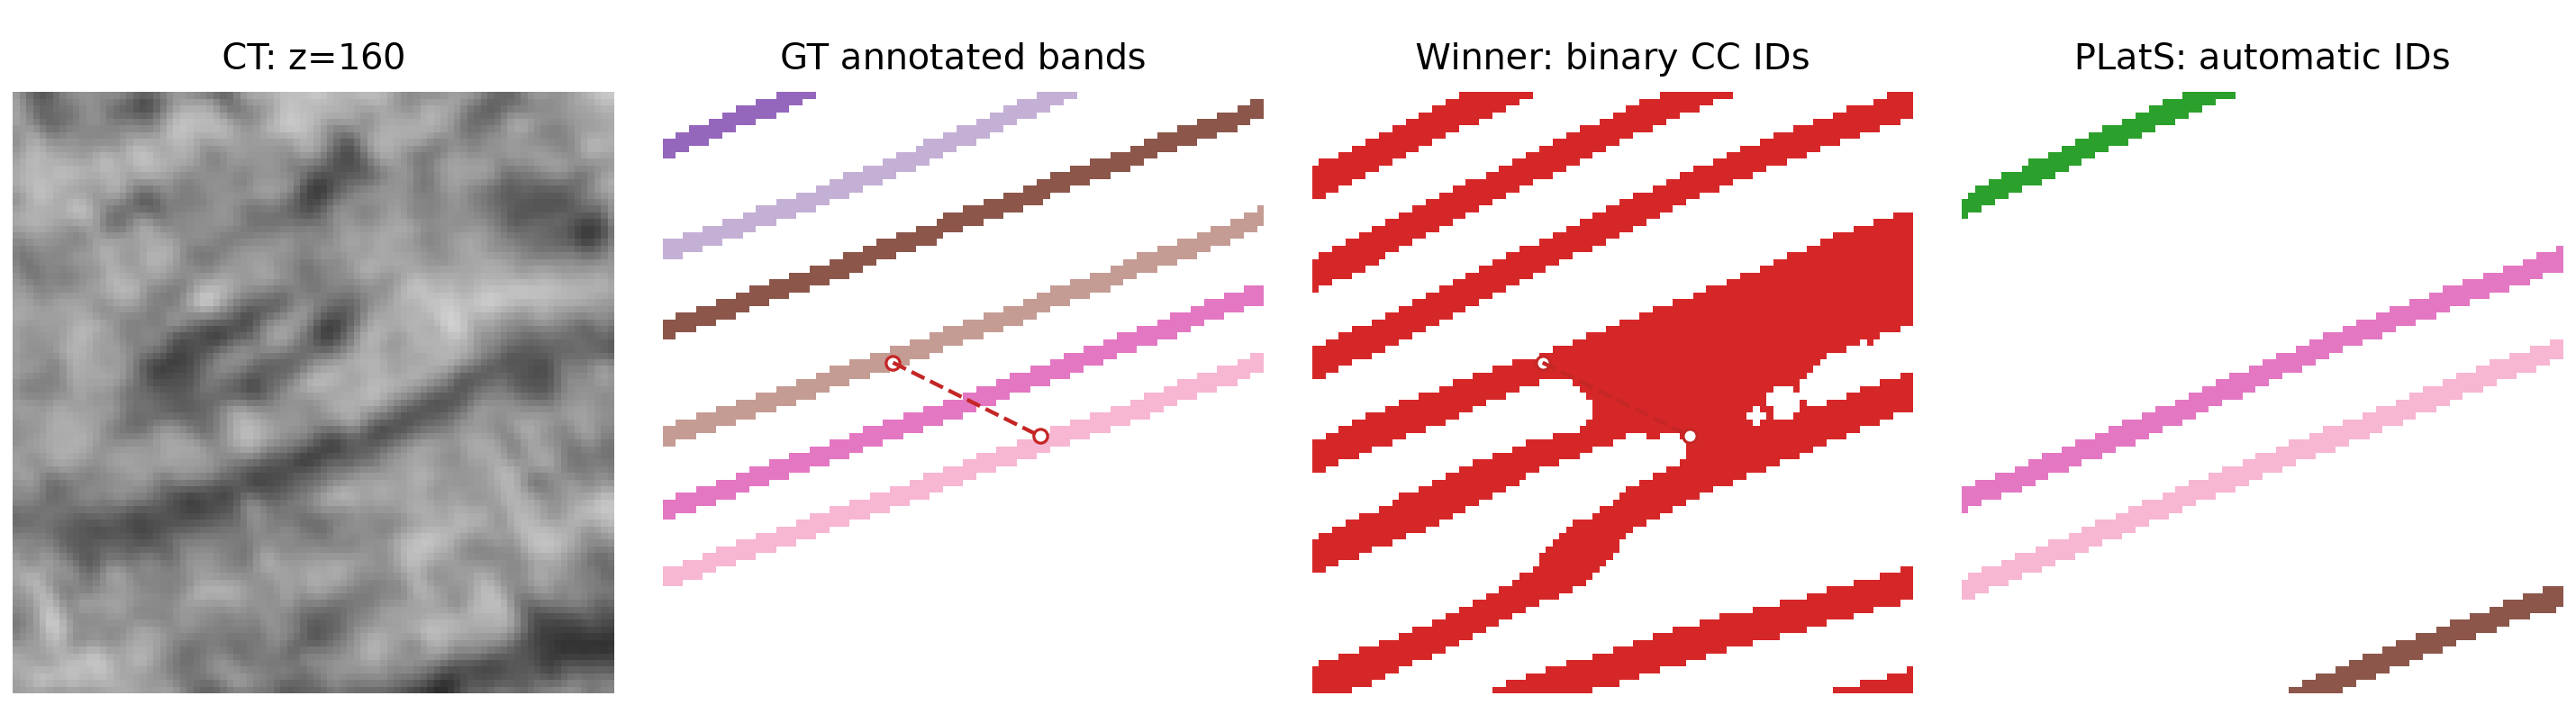
\includegraphics[width=\textwidth]{figures/binary_failure_zoom.png}
 \caption{Enlarged native slice from the main-paper binary failure
 example: the same $90\times90$-pixel crop at TIFF $z=160$ in all four columns.
The winner component connects distinct GT bands; automatic PLatS has lower
 coverage. Twenty-seven predicted voxels in the sampled gap are known background;
 none of its 34 samples are ignored. The red dashed segment marks this sampled
 gap in GT and winner panels. Labels are displayed without dilation or smoothing.}
\end{figure*}

\section{Large pages and spiral-fitting integration}
\begin{table*}[t]
\centering
\small
\setlength{\tabcolsep}{4pt}
\begin{tabular}{lrrrrr}
\toprule
Page & Area cm$^2$ & Accepted/attempted & Join median (vox) & Target median & Target p90 \\
\midrule
page\_a & 5.67 & 255/365 & 1.181 & 3.905 & 15.856 \\
page\_b & 8.92 & 411/565 & 1.361 & 2.778 & 15.234 \\
\bottomrule
\end{tabular}
\caption{0058 large-page outputs. Areas are reconstructed mesh areas; joins include accepted windows only. Target distances exclude reference-boundary samples and are measured after all ink outputs are frozen.}
\label{tab:largepages}
\end{table*}

The large-page main-paper figure uses \emph{0058} on the same two preselected
PHerc0139 regions as our earlier downstream control. Native sampling is
9.362~\textmu m; patch size 320 and step 128 give 60\% linear overlap.
The first decoded prediction defines a tangent frame; later points come from
accepted predictions. An overlap acceptance gate can reject ambiguous growth,
so accepted join error is conditional on acceptance and is not a global
geometric error. Independent SLIM retains holes in predicted chart support.
The inward normal is fixed from the scroll umbilicus before ink inference;
full inward/outward PNGs are preserved. Geometry and partial ink labels enter
only after all reconstruction/ink hashes are frozen. The known ink-model scroll
and potentially overlapping external training regions are not held-out
transcription tests.
On page A, the single-method supported-pixel ink AP/Dice are 0.9170/0.8294;
labeled coverage is 17.37\% and delivered Dice is 0.2932. These supported pixels
are not the common-pixel set used in the integration comparison below.

An earlier integration pilot, using original \emph{0076}, compares the direct
prediction, published m7 tracks passed to the official spiral fitter, PLatS
patches alone, and tracks plus PLatS patches. All fits have the same 30,000-step
budget, canonical initialization, independent flattening and frozen ink.
The published tracks have \emph{unverified Kaggle-winner provenance}; this is
not the first-place model comparison. Two predicted local charts alone leave
global fitting underconstrained. We retain these controls to demonstrate an
integration route, not an upper bound on the published fitting method.

\begin{table*}[t]
\centering
\small
\setlength{\tabcolsep}{4pt}
\begin{tabular}{lrrrrrrr}
\toprule
Input/method & Area cm$^2$ & Median vox & p90 vox & Ink AP & Ink Dice & Coverage & Delivered Dice \\
\midrule
Direct PLatS & 6.258 & 2.249 & 8.059 & 0.7582 & 0.6021 & 0.2348 & 0.3324 \\
Published tracks & 5.773 & 14.450 & 29.358 & 0.3314 & 0.1731 & 0.1598 & 0.0524 \\
PLatS patches only & 6.236 & 6.311 & 94.290 & 0.8393 & 0.7446 & 0.1444 & 0.1314 \\
Tracks + PLatS & 5.948 & 3.112 & 12.187 & 0.9881 & 0.9336 & 0.1591 & 0.2239 \\
\bottomrule
\end{tabular}
\caption{Original 0076 integration pilot on page A. Common ink uses identical pixels across all four arms; coverage and delivered Dice expose missing output. Published tracks are not verified as the Kaggle winner.}
\label{tab:spiralintegration}
\end{table*}

\begin{figure*}[t]
 \centering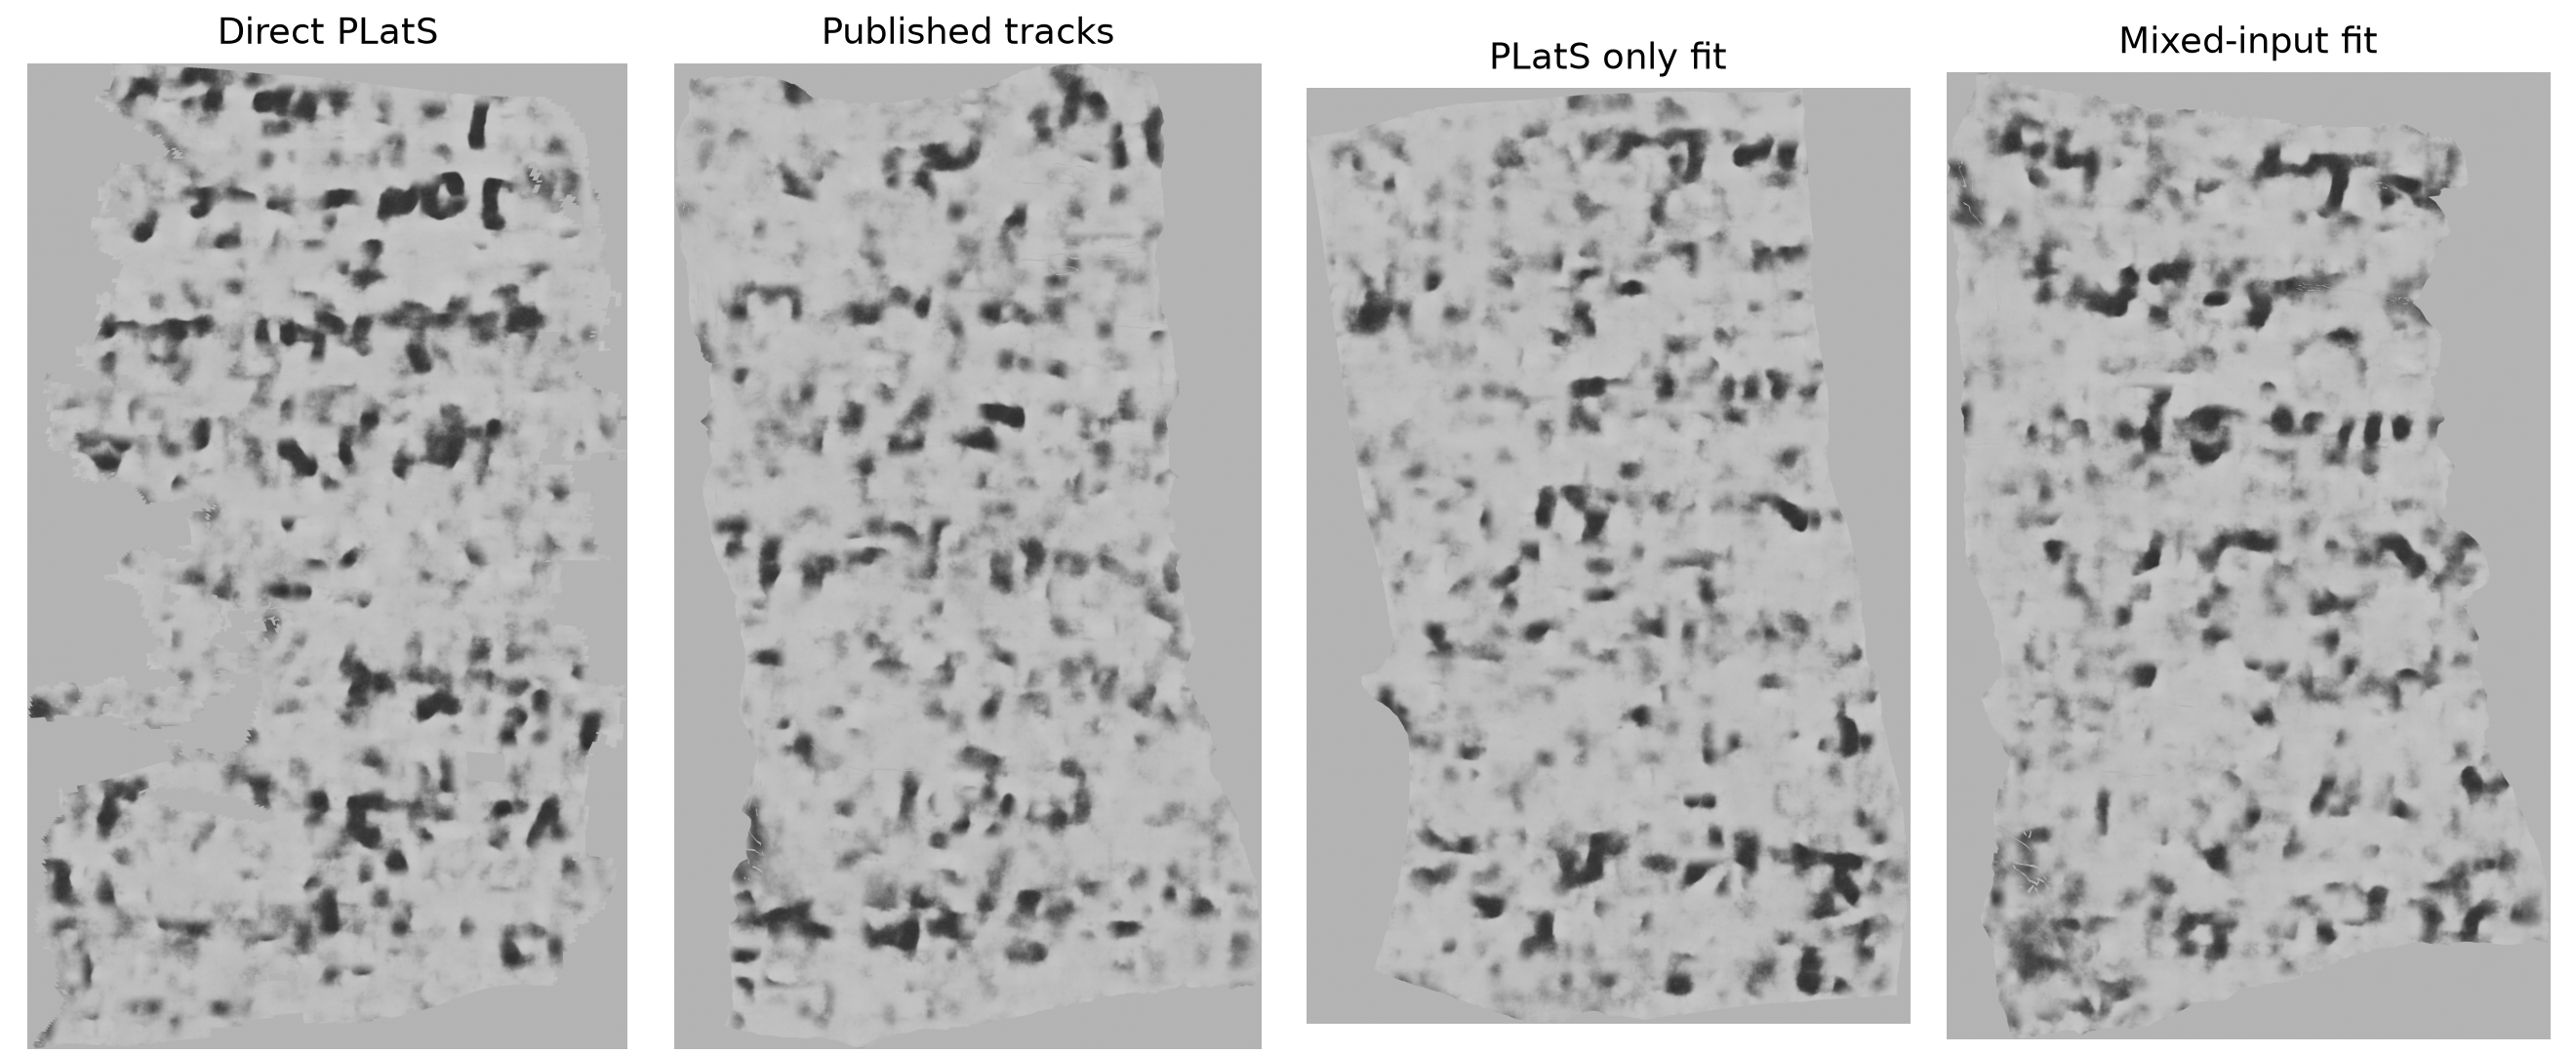
\includegraphics[width=\textwidth]{figures/spiral_integration.png}
 \caption{Large-page spiral integration control on PHerc0139 page A, original
 0076 (Supplementary only). Direct prediction, published-track fitting,
 prediction-only fitting and mixed-input fitting all use independent layouts
 and the same ink model. The track source is not verified as the Kaggle winner.}
 \label{fig:spiral}
\end{figure*}
Ink AP and Dice in Table~\ref{tab:spiralintegration} use the same 26,296
fully supported labeled pixels across all four arms. Labeled coverage and
``delivered'' Dice also count missing output, assigning zero to missing
predictions. Pairwise comparisons use different common pixel sets and must
not be mixed with the all-arm table. Page B has no audited ink labels.
High common-pixel scores on a small delivered fraction do not establish
whole-page letter recovery. This pilot studies integration and drift.
